\chapter{Interfaccia dell'applicazione}
\label{sec:Interfaccia dell'applicazione}
L'applicazione si compone di 2 schermate, la prima per impostare i dati della simulazione e attraverso il tasto "SIMULA" è possibile passare alla seconda schermata che contiene i risultati della simulazione.

\begin{figure}[h]
\centering
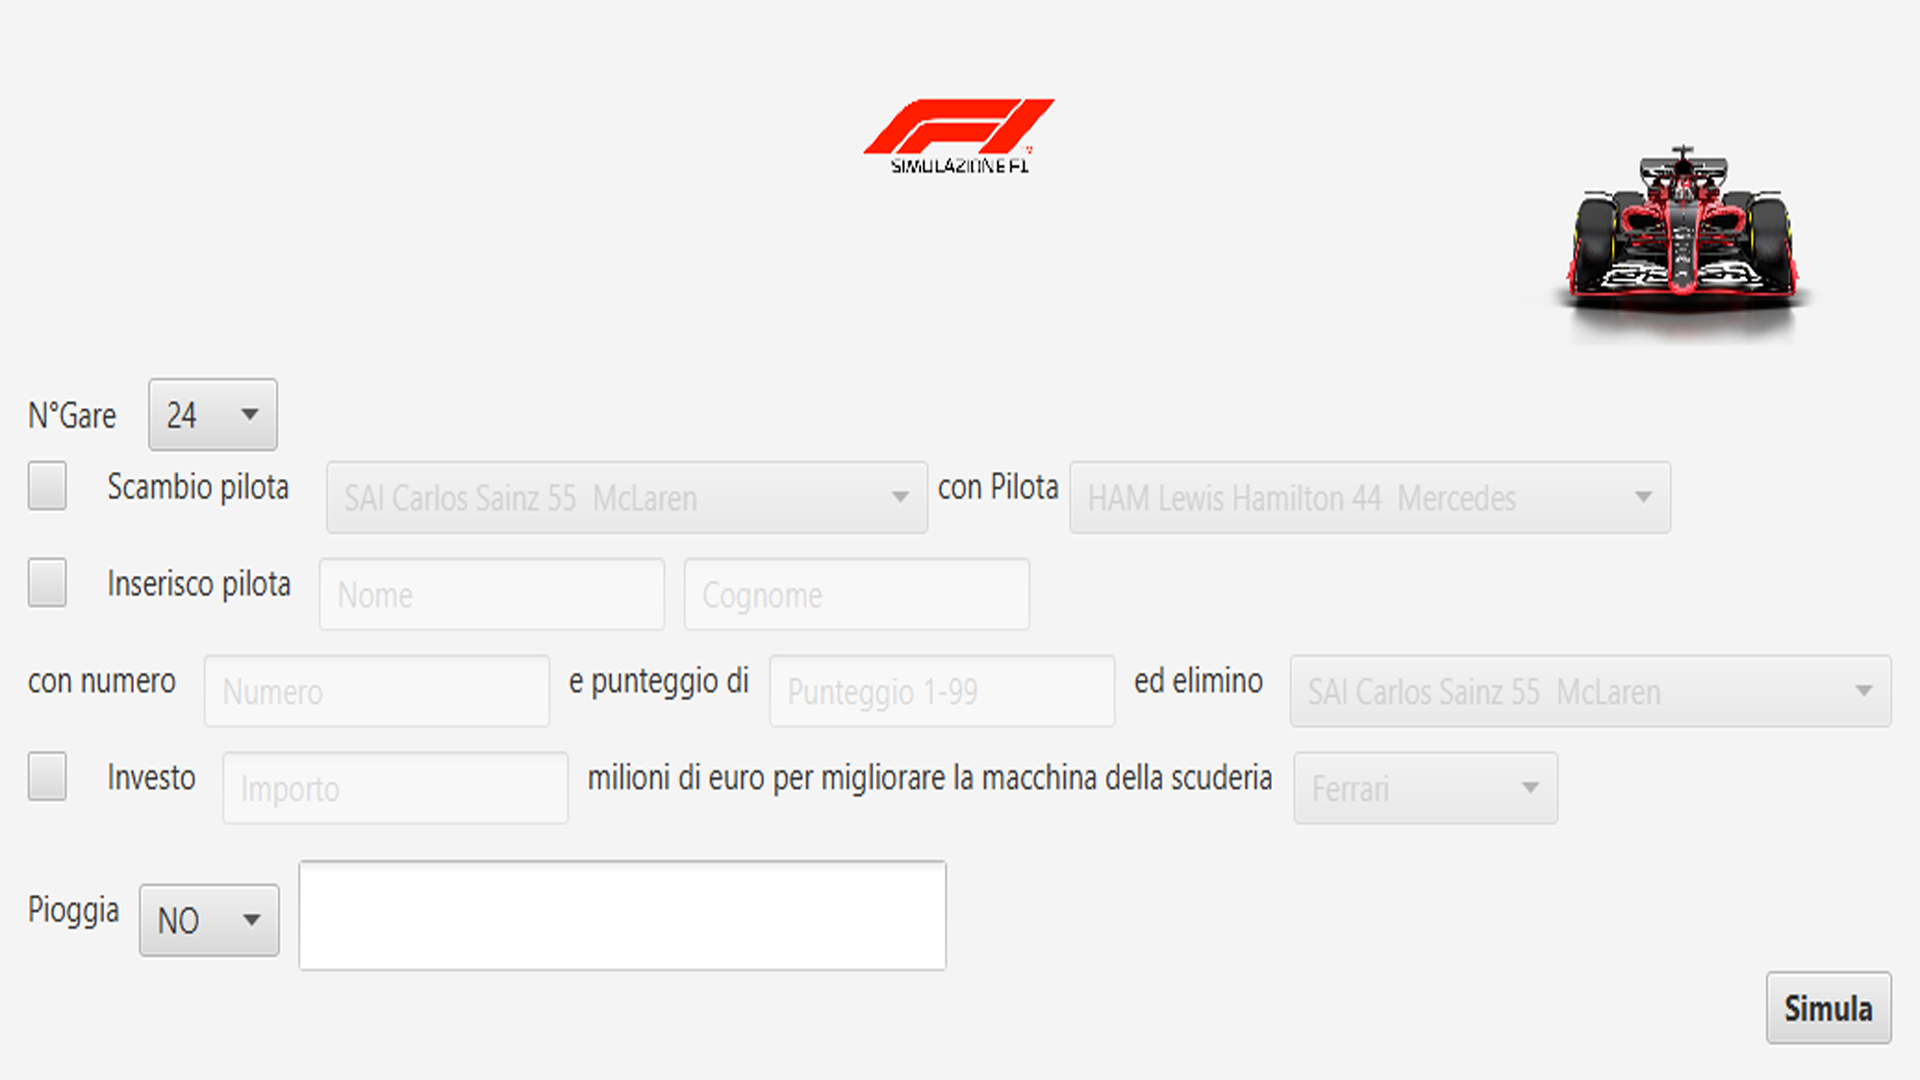
\includegraphics[width=1\linewidth]{images/Schermata impostazione simulazione senza dati.png}
\caption{Schermata impostazione della simulazione}
\label{fig:Schermata impostazione della simulazione}
\end{figure}

\begin{figure}[h]
\centering
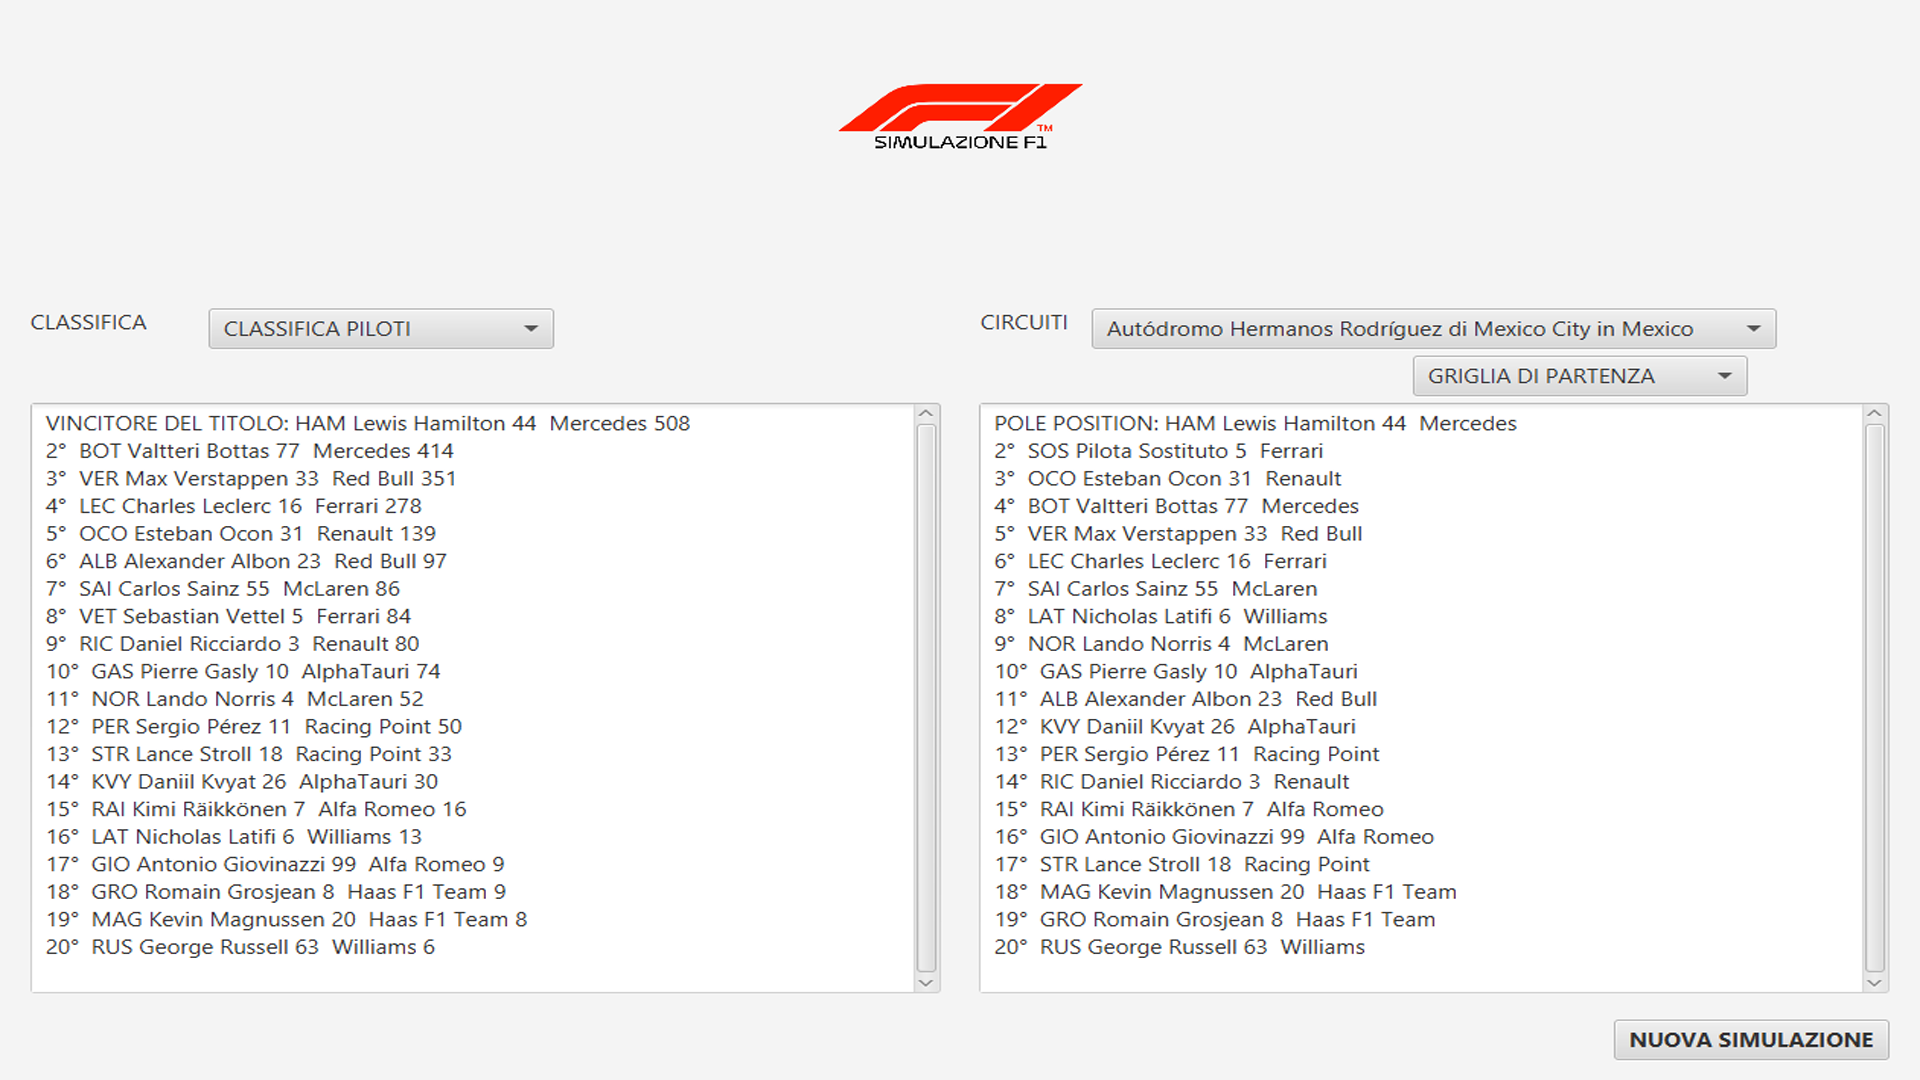
\includegraphics[width=1\linewidth]{images/Risultati piloti.png}
\caption{Classifica Piloti e griglia di partenza della gara in Messico}
\label{fig:Classifica Piloti e griglia di partenza di una gara}
\end{figure}

\begin{figure}[h]
\centering
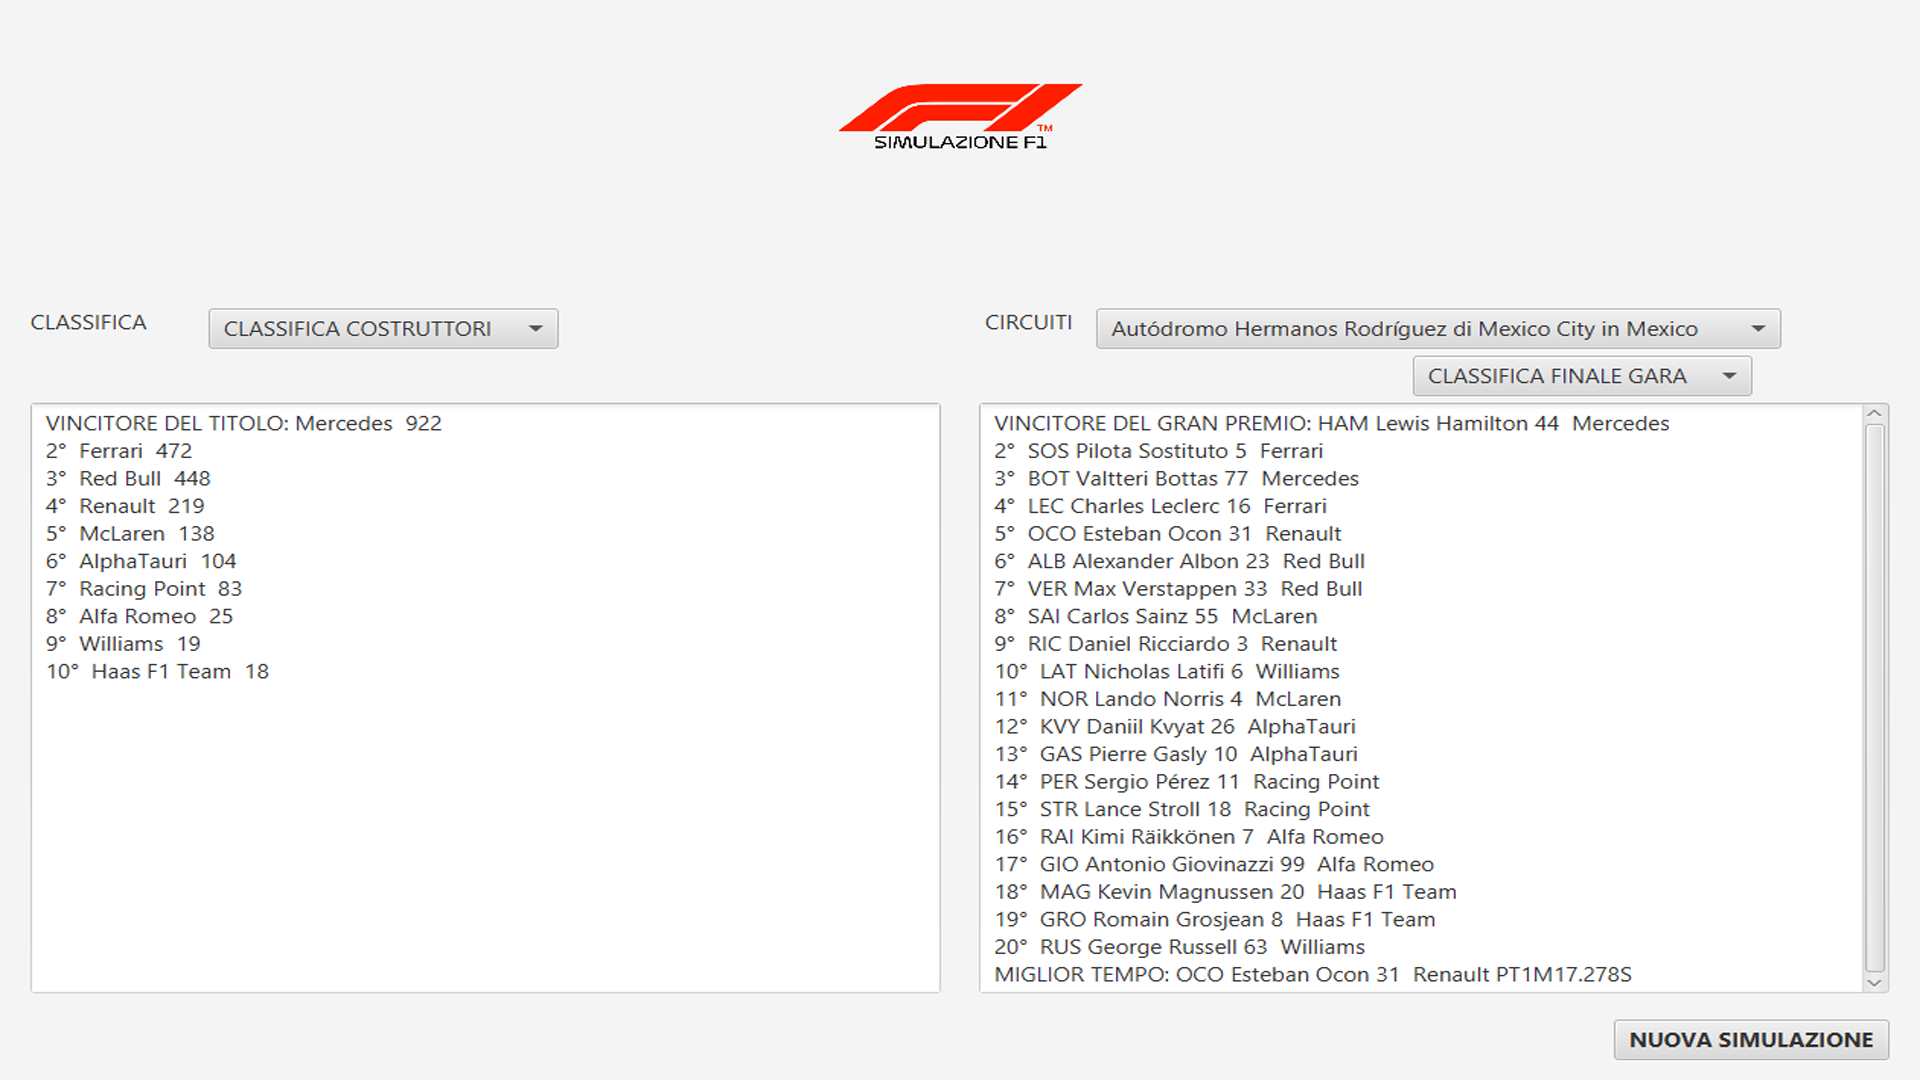
\includegraphics[width=1\linewidth]{images/Risultati scuderia.png}
\caption{Classifica Scuderia e classifica finale della gara in Messico}
\label{fig:Classifica Scuderia e classifica finale di una gara}
\end{figure}

\begin{figure}[h]
\centering
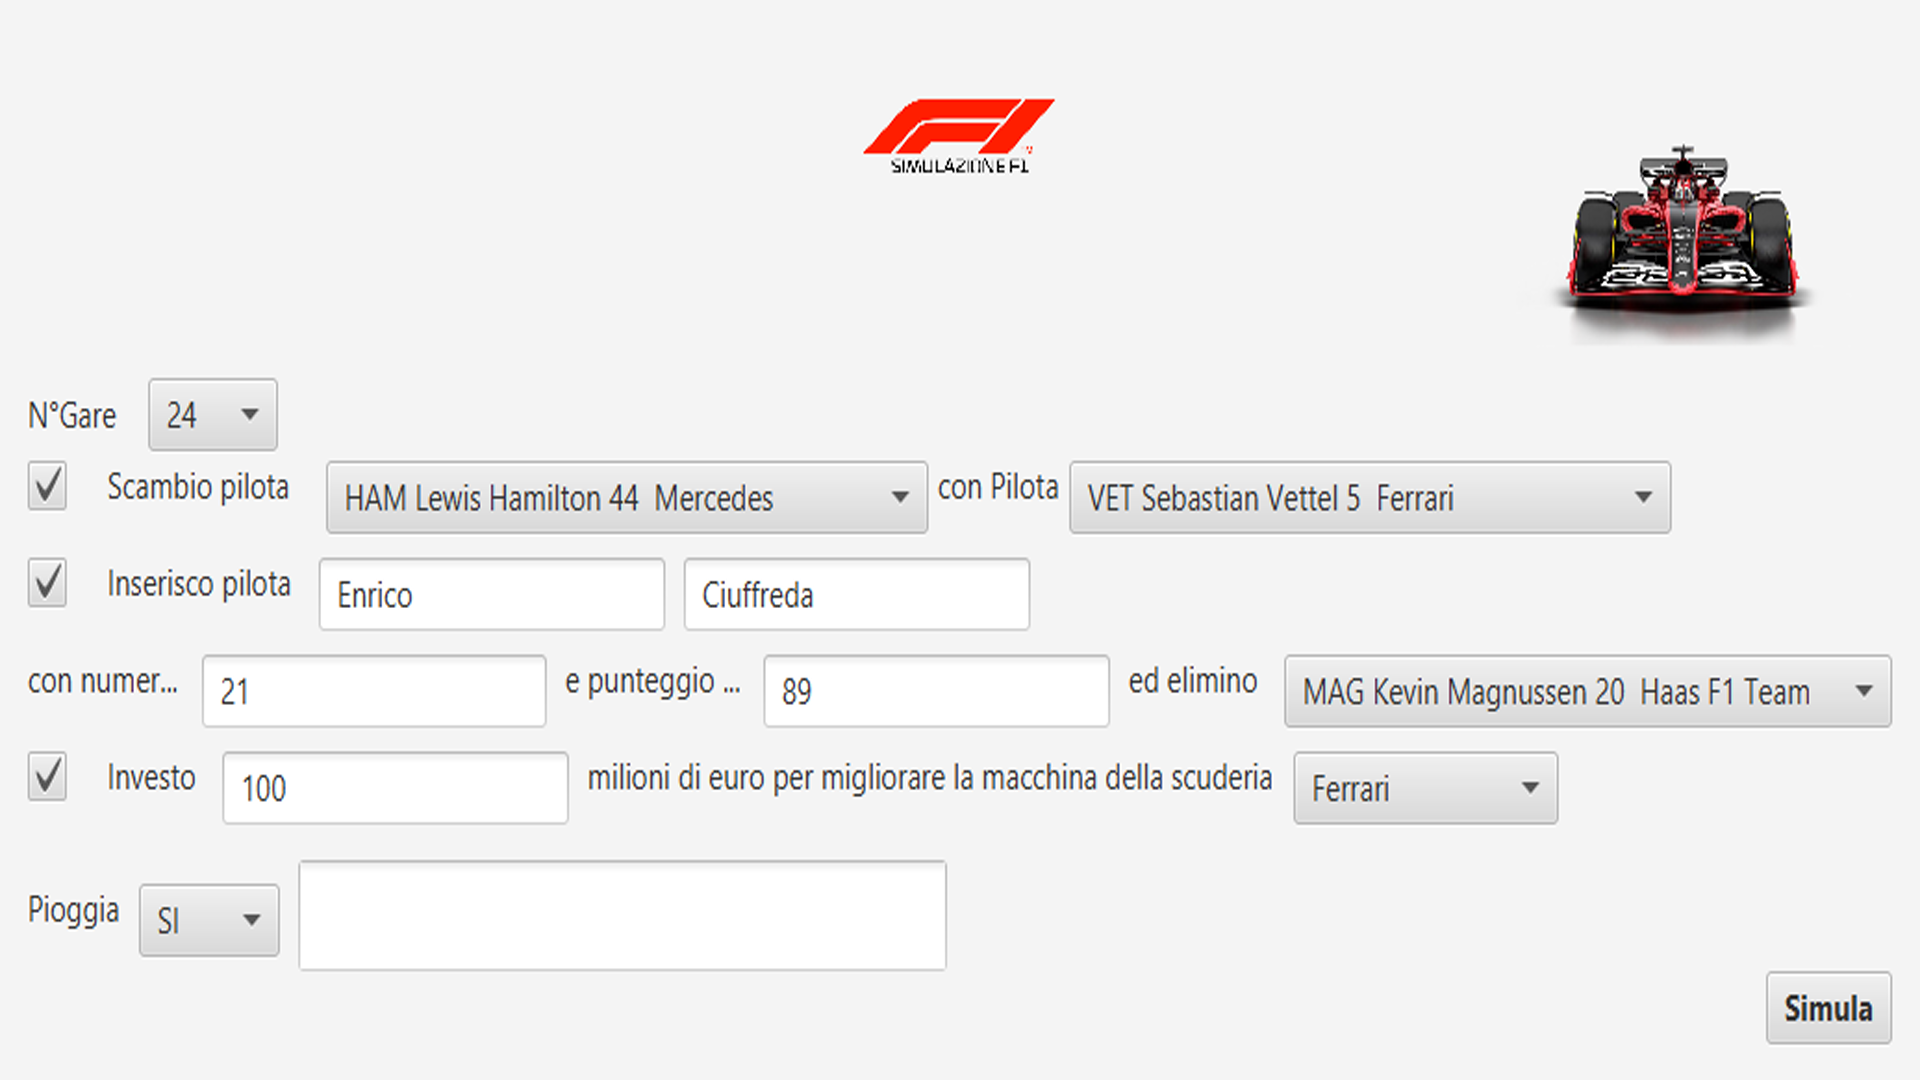
\includegraphics[width=1\linewidth]{images/Schermata impostazione simulazione con dati.png}
\caption{Schermata impostazione della simulazione con dati scelti dall'utente}
\label{fig:Schermata impostazione della simulazione con dati scelti dall'utente}
\end{figure}

\begin{figure}[h]
\centering
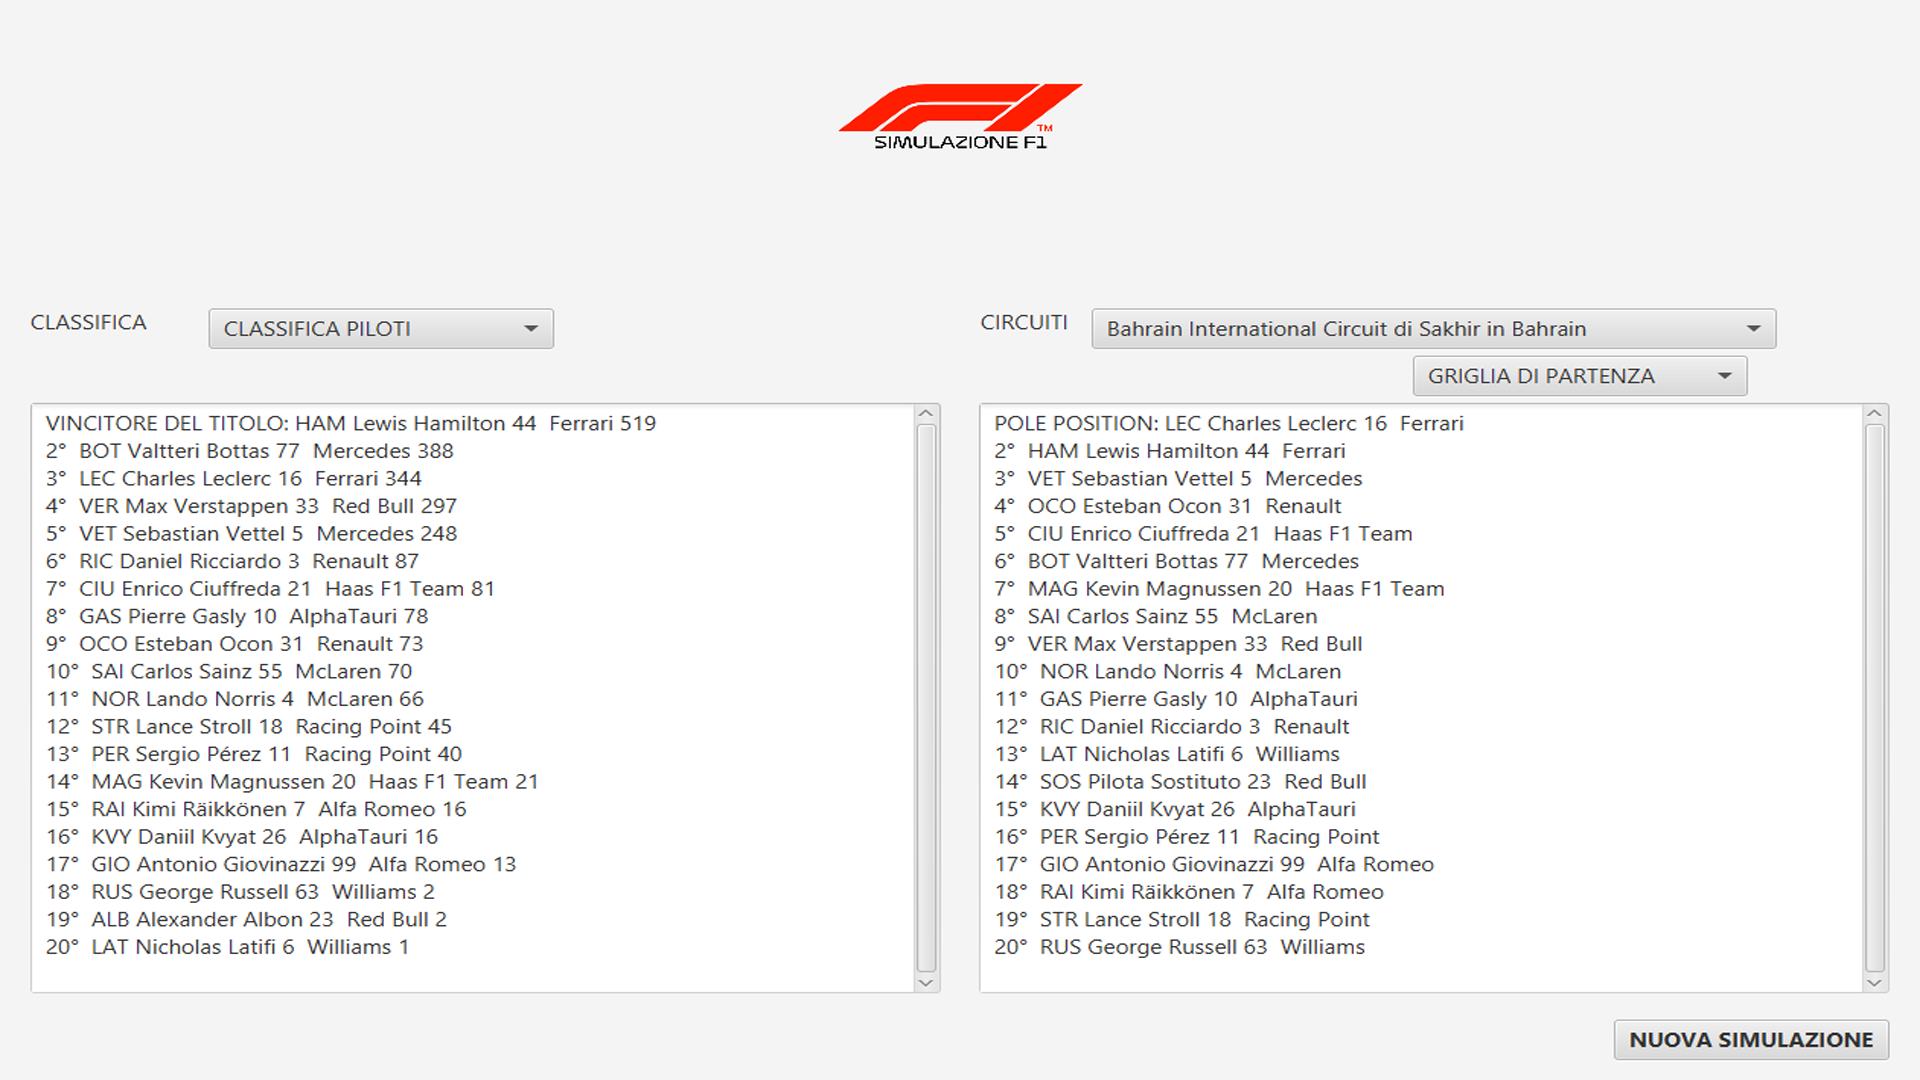
\includegraphics[width=1\linewidth]{images/Risultati ottenuti con impostazioni scelte dall'utente.png}
\caption{Classifica Piloti e griglia di partenza della gara in bahrein}
\label{fig:Classifica Piloti e griglia di partenza di una gara}
\end{figure}

\begin{figure}[h]
\centering
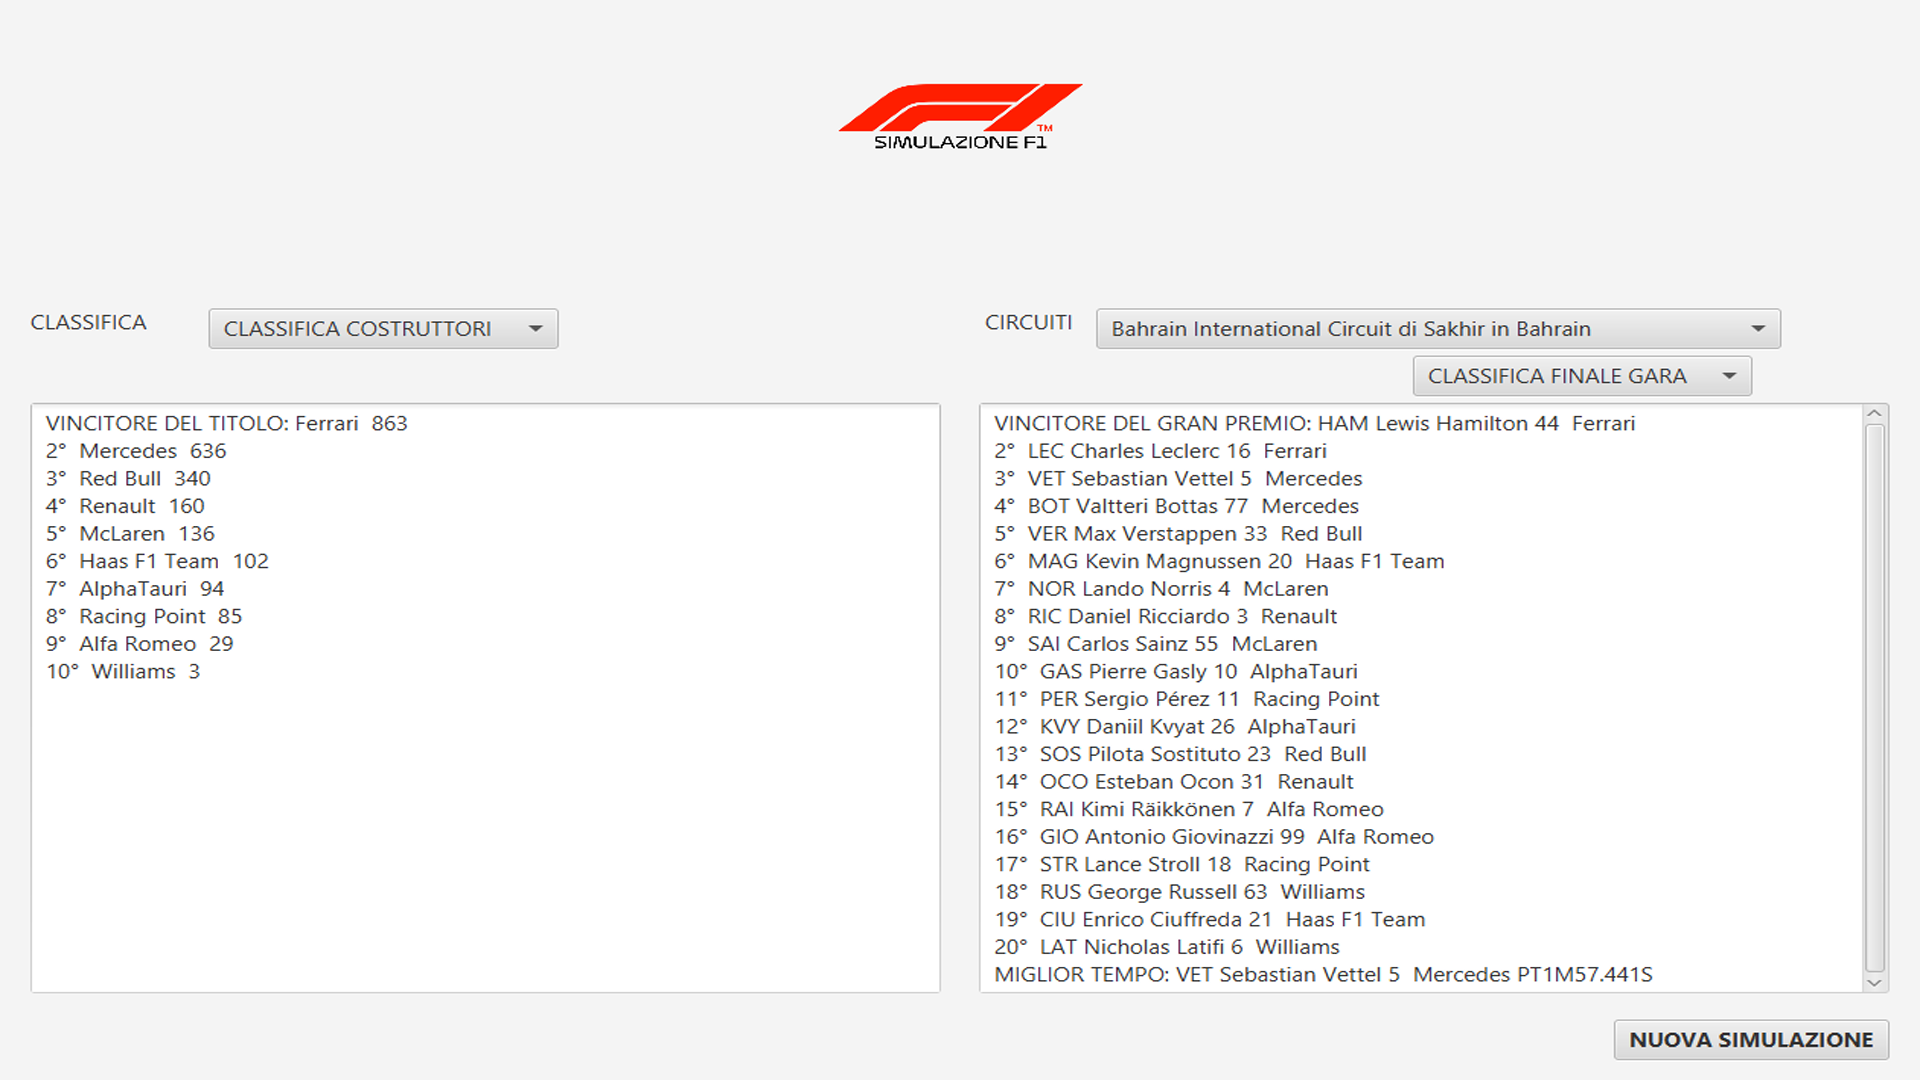
\includegraphics[width=1\linewidth]{images/Risultati scuderia ottenuti con impostazioni scelte dall'utente.png}
\caption{Classifica Scuderia e classifica finale della gara in bahrein}
\label{fig:Classifica Scuderia e classifica finale di una gara}
\end{figure}